\documentclass[a4paper, 12pt]{report}

% Packages
\usepackage[utf8]{inputenc}
\usepackage[T1]{fontenc}
\usepackage[french]{babel}
\usepackage{graphicx}
\usepackage{float}
\usepackage{hyperref}
\usepackage{fancyhdr}
\usepackage{titlesec}
\usepackage{lipsum}

% Mise en page
\pagestyle{fancy}
\fancyhf{}
\setlength{\headheight}{15pt}
\renewcommand{\headrulewidth}{0.5pt}
\renewcommand{\footrulewidth}{0pt}
\lhead{\leftmark}
\rhead{\thepage}
\renewcommand{\chaptermark}[1]{\markboth{\MakeUppercase{#1}}{}}
\titleformat{\chapter}[display]{\normalfont\huge\bfseries}{\chaptertitlename\ \thechapter}{20pt}{\Huge}
\graphicspath{ {./images/} }

% Informations du document
\title{Test Rapport de projet d'électronique pour système embarqué}
\author{Simon GIRARD - Dimitri TIMOZ - Mathis SAUNIER - Alix ANNERAUD}
\date{\today}

\begin{document}

% Page de garde
\begin{titlepage}
\maketitle{}
\end{titlepage}

% Table des matières
\tableofcontents

% Chapitres
% An introduction with the project objectives
\chapter{Introduction}
\lipsum[1-2]
% 
\chapter{Contexte}
\lipsum[3-4]

\chapter{Conception}

% A complete fritzing circuit with all the wiring of the different sensors, actuators and components for display
% + A detailed explanation of your wiring choices as well as any additional technical choices (power, use of resistors, diodes, etc.)
% + A detailed explanation of the chosen components role and operating principle
\section{Electronique}
\subsection{Choix des composants}
\subsection{Cablâge des composants}
\subsection{Schéma EasyEDA}
% A detailed section of your code: approach, structure, etc.
\section{Code}
\subsection{Architecture du programme}
\subsection{Développement des fonctions métiers du robot}
% Là je sais pas mais on pourrait faire les fonctions des roues, l'algo pour le chemin, le multi threading, le code pour le son ...

\subsection{Développement de l'interface de contrôle}
Nous avons décidé de nous tourner vers les technologies web pour développer l'interface de contrôle de notre robot. Celles-ci, par leur simplicité, nous ont permis d'avancer rapidement, et de nous concentrer plutôt sur le développement des fonctionnalités de notre robot. Les navigateurs offrent notamment un large support des manettes de jeux, et son intégration a donc été très simple.
Le robot fait tourner un serveur HTTP afin de recevoir les commandes du client. Internet étant accessible à travers le wifi de l'INSA, le robot peut donc être controlé à distance dans tout le périmètre de l'école. Disposant d'une caméra, il est possible de s'aider du flux vidéo pour contrôler le robot.
Néanmoins, le réseau de l'INSA nous faire subir quelques instabilités. Si la latence est très satisfaisante le plus souvent, il arrive au robot de perdre la connexion avec le client pendant quelques secondes. Ces problèmes de perte de contrôle du véhicule peuvent se révéler très problématiques. Nous désignons la DSI comme responsable d'éventuels accidents.
L'interface web nous a été très utile pour piloter le robot, mais aussi pour expérimenter avec différents paramètres, ainsi que pour visualiser l'état de certains capteurs. La plupart des paramètres et affichages des entrées ont été supprimées aujourd'hui.

\section{Mécanique}
\subsection{Choix de la taille des roues}
\subsection{Emplacement des roues et des capteurs}
Notre robot a connu beaucoup d'évolution tout au long du projet que cela soit au niveau du code ou de l'organisation des composants.
\\
Initialement, nous avions placé les roues à "l'arrière du chassis" (à l'opposé de l'emplacement du capteur de distance) avec une roue folle vers l'avant. Cette disposition des roues convenait très bien à la conduite manuelle du robot car elle permettait une rotation rapide de l'avant. Cependant, nous avons également eu beaucoup de changement concernant le choix de nos capteurs de lignes (cf 3.1.1 et 5.1.3) et nous avons remplacé des capteurs placés sous le chassis par un autre placé tout à l'avant. La rotation rapide de notre robot est ainsi devenue un problème, pertubant les données captées par notre capteur à l'avant. De plus, la position reculée des roues faisait que le centre de pivot de notre robot était également reculé, et par conséquent, éloigné de notre capteur suiveur de ligne. C'est pour l'ensemble de ces raisons que nous avons finalement adapté la position de nos roues en les plaçant à l'avant, avec notre capteur.
\\
Ce changement nous a permis de meilleurs résultats sur l'algorithme du suiveur de ligne tout en gardant une maniabilité sensiblement inchangée pour le mode manuel.
% A section with detailing each member’s taks in the project + l'organisation interne
\chapter{Méthodologie}
\lipsum[5-6]

\chapter{Résultats}
\lipsum[7-8]
\section{Difficultés rencontrées}
\subsection{Problèmes de son}
Au tout début du projet nous avons eu l'idée d'ajouter un haut-parleur à notre robot. L'idée était très simple : utiliser le port jack intégré à notre Raspeberry Pi pour émettre un son qui sera ensuite amplifié avant d'être émis par un haut-parleur. En fin de compte, cette fonctionnalité a été un vrai challenge à ajouter sur notre robot et c'est pour cete raison que nous y dédions une sous-partie du rapport. Nous détaillerons toutes les solutions essayées ainsi que la solution finalement retenue.
\\
La première solution censée apporter le son à notre robot a été le module d'amplification suivant : 386AMP from DFRobot
\\
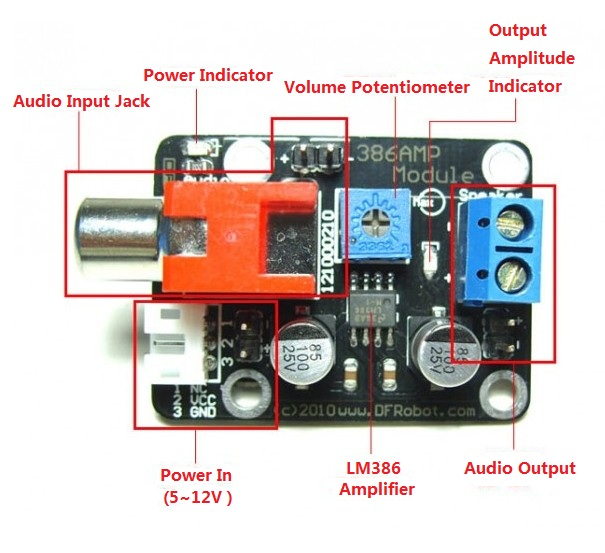
\includegraphics[scale=0.5]{386AMP.jpg}
\\
Cependant, il nous fallait un câble jack 3.5 vers RCA afin de pouvoir utiliser le module d'amplification sur lequel pouvait ensuite être aisément branché un haut-parleur. Étant donné que le laboratoire d'électronique ne possédait pas ce type de câble, nous avons fini par trouver le matériel nécessaire chez nous. Ainsi, nous avons pu faire les premiers tests du module avec nos téléphones. Ces derniers étant concluants, nous avons recherché les commandes nécessaires à la lecture d'un audio sur Raspeberry. Nous utilisons donc 3 fonctions systèmes
de la Raspeberry.
\begin{itemize}
    \item system("amixer -q set PCM,0 unmute"); permet de s'assurer que le son de la Raspeberry est actif
    \item system("mpg321 -q assets/" + filename + " \&"); permet de lancer, en processus d'arrière plan, l'audio désigné par la variable filename
    \item system("pkill -9 mpg321"); permet d'arrêtter le processus qui joue la musique en cours
\end{itemize}
Malheureusement, lors de notre premier test du module d'amplification sur la Raspeberry nous n'avons obtenu qu'un bip continu. Ce problème survient uniquement lorsque les autres fonctionnalités  de notre robot était en marche. Un autre groupe a été confronté à ce problème et malgré nos efforts communs et les nombreux cas similaires présents sur Internet nous n'avons jamais réussi à utiliser le module d'amplification.
\\
Les solutions que nous avons essayées sont pourtant nombreuses :
\begin{itemize}
    \item changement de configuration d'amixer (le logiciel gérant le son sur la Raspeberry)
    \item changement de matériel (module d'amplification et câble)
    \item changement de configuration du PWM (dont l'activation semble être à l'origine de notre problème)
\end{itemize}
En fin de compte, après l'échec de toutes ces solutions, c'est l'utilisation du MAX 98357A, un Amplifier/DAC (Digital Analog Converter), qui nous a permis de jouer des sons sur notre robot. Nous en avons donc conclu que le port jack de la Raspeberry était bien à l'origine de notre problème sans pour autant l'avoir résolu.

\subsection{Tentative d'algorithme suiveur de ligne PID}
Nous avons réalisé quelques recherches sur des algorithmes permettant de faire de l'asservissement et nous nous sommes rendus compte que l'algorithme le plus répendu est le PID Control.
L'objectif de cet algorithme est de faire en sorte que l'erreur entre la position actuelle du robot et la position désirée soit nulle. Pour cela, il faut calculer l'erreur, c'est à dire la différence entre la position actuelle et la position désirée, puis calculer la dérivée de cette erreur et enfin calculer l'intégrale de cette erreur.
Sur le papier, cet algorithme semble très simple à mettre en place. Cependant, nous avons rencontré de nombreuses difficultés lors de la mise en place de cet algorithme.
En effet, nous avons dû faire face à de nombreux problèmes de détection de ligne. En effet, nous avons essayé de faire fonctionner notre robot avec des capteurs QTR mais ces derniers ne fonctionnaient pas correctement. Nous avons donc essayé de faire fonctionner notre robot avec une caméra mais celles-ci n'avait pas un angle de vue assez large pour détecter la ligne suffisament loin pour le PID.

\subsection{Échec des capteurs QTR}
Nous avons essayé d'utiliser des capteurs QTR pour détecter la ligne. Cependant, nous avons rencontré de nombreux problèmes avec ces capteurs. En effet, nous n'avons rien trouvé sur internet qui nous permettait de les utiliser correctement avec un raspberry.
Nous avons donc développé notre propre code pour utiliser ces capteurs. Cependant, nous n'avons pas réussi à obtenir des résultats satisfaisants avec ces capteurs. En effet, ils détectaient trop de bruit et ne détectaient pas la ligne de manière fiable.
Nous ne savons pas si le problème venait de notre code ou des capteurs eux-mêmes mais nous avons finalement décidé de ne pas utiliser ces capteurs.
Nous nous sommes dit que le seul moyen de faire fonctionner notre robot correctement était d'utiliser une caméra. En effet, en observant une seule bande de pixel sur une image, nous pouvions détecter la ligne de manière fiable.


\subsection{Retours d'expériences}
% Partie dans laquelle on revient sur ces difficultés, on essaie de les raisonner
% (leur trouver une raison) et faire comme si le projet avait été une source incroyable d'apprentissage pour nous
\section{Les capacités du robot}

\chapter{Conclusion}
\lipsum[9-10]

% Bibliographie
\begin{thebibliography}{9}
\bibitem{latexcompanion} 
Michel Goossens, Frank Mittelbach, and Alexander Samarin. 
\textit{The \LaTeX\ Companion}. 
Addison-Wesley, Reading, Massachusetts, 1993.

\bibitem{einstein} 
Albert Einstein. 
\textit{Zur Elektrodynamik bewegter K{\"o}rper}. (German) 
[\textit{On the electrodynamics of moving bodies}]. 
Annalen der Physik, 322(10):891–921, 1905.

\bibitem{knuthwebsite} 
Knuth: Computers and Typesetting,
\\\texttt{http://www-cs-faculty.stanford.edu/\~{}uno/abcde.html}
\end{thebibliography}

\end{document}
